%!TEX root = ../AutoML-fuer-Segmentierung.tex
\chapter{Auto-DeepLab}
\label{ch:autodeeplab}

% Einträge in die ToDo-Liste setzen (für Änderungen muss 2 mal übersetzt werden, wie bei TOC auch)
\todo{Deeplab mit Inhalt füllen}

\section{Funktionsweise / Theorie}

Auto-DeepLab ist ein NAS Programm, welches im Jahr 2019 zur Segmentierung von Bildern entwickelt wurde. Die folgenden Ausführungen zur Funktionsweise des Programms beruhen auf dem Paper \cite{autodeeplabPaper} von Chenxi Liu et al.\\
Auto-DeepLab verfolgt den Ansatz, die Netzstruktur sowie die Zellstruktur des Convolutional Netzes zu suchen. Die Architektur kann mittels Gradient Descent in 3 GPU Tagen gesucht werden. Anders als bei nicht-differenzierbaren Suchtechniken arbeitet Auto-DeepLab somit sehr effektiv: Es wird nicht in einer diskreten Menge von Kandidaten nach der besten Architektur gesucht. Stattdessen wird mit Hilfe von Gradient Descent (also mittels Differenzierbarkeit, also stetig) gearbeitet. Die Optimierung geschieht in Hinblick auf die Validierungsperformance. Diese Effektivität ist auch notwendig, da Bildsegmentierung auf hochauflösenden Bildern funktionieren muss und auch das segmentierte Ausgabebild im besten Fall die gleiche Auflösung wie das zu segmentierende Eingabebild haben sollte.\\
Zum Zeitpunkt der Veröffentlichung von Auto-DeepLab war der Stand der Entwicklung der NAS Programme so, dass oft nur das Innere der Zellen automatisiert gesucht wurde und dann anhand dieses Resultates das Netz bestimmt wurde. Hier unterscheidet sich Auto-DeepLab, da sowohl Netz als auch die Zellstruktur automatisiert ermittelt werden.
Im Folgenden wird die Suche im hierarchischem Suchraum beschrieben. Wir beginnen mit dem Suchraum bezüglich des Zellinneren.\\[0.3cm]
Zunächst einmal definieren wir, was eine Zelle ist:\\
Eine Zelle ist ein gerichteter, azyklischer Graph, der aus einer geordneten Sequenz aus n Knoten besteht. Jeder Knoten ist hierbei ein sogenannter Block. Mehrere Zellen miteinander verkettet bilden dann das gesamte neuronale Netz.\\
Die Blöcke in den Zellen sind Strukturen, die zwei Tensoren als Input entgegennehmen und einen Output-Tensor ausgeben. Block $i$ in Zelle $l$ kann mit einem 5-Tupel charakterisiert werden: $(I_1, I_2, O_1, O_2, C)$ mit $I_1, I_2 \in \mathcal{I}_{i}^{l}$, wobei $\mathcal{I}_{i}^{l}$ die Menge aller möglichen Input-Tensoren darstellt: $\mathcal{I}_{i}^{l}$ besteht aus dem Output der vorherigen Zelle, $H^{l-1}$, dem Output der Zelle zwei Zellen vor der aktuellen Zelle $l$, $H^{l-2}$, und jeweils dem Output der Blöcke der aktuellen Zelle, die sich in dem gerichteten, azyklischen Graphen vor dem aktuellen Block i befinden: $H_{1}^{l}, ... , H_{i-1}^{l}$. Dadurch haben die Blöcke einer Zelle, die im gerichteten Graphen weiter hinten sind, mehr mögliche Inputs.\\
Zurück zu dem charakterisierenden 5-Tupel bilden $O_1$ und $O_2$ die Layer-Typen jeweils für die beiden Inputs $I_1$ und $I_2$ mit $O_1, O_2 \in \mathcal{O}$. Die Menge $\mathcal{O}$ besteht wiederum aus 8 möglichen Operatoren: 3 x 3 depthwise-separable conv, 5 x 5 depthwise-separable conv, 3 x 3 atrous conv with rate 2, 5 x 5 atrous conv with rate 2, 3 x 3 average pooling, 3 x 3 max pooling, skip connection, no connection (zero). Das $C$ stellt den Operator dar, mit dem die beiden auf die Layers angewandten Inputs zu einem Output gemacht werden: $O_{1}(I_{1})$ und $O_{2}(I_{2})$ werden immer einfach elementweise addiert. Damit könnte man die Charakterisierung eigentlich auch auf ein 4-Tupel bestehend aus $I_1, I_2, O_1, O_2$ beschränken.\\
Der Outpur Tensor der Zelle $i$, $H^l$, ist einfach die Konkatenation von $H_{1}^{l}, ..., H_{n}^{l}$. D.h. die Outputs der Blöcke der Zelle i werden konkateniert in der Reihenfolge des Auftreten im Graphen.\\[0.3cm]
Nachdem die Struktur der Zellen nun erklärt ist, fahren wir fort mit der Beschreibung, wie sich die Architektur des Netzes zusammenstellt. Dies ist am besten graphisch mit Abbildung \ref{pic:autodeeplab_Architektur} möglich.\\
Links in Abbildung \ref{pic:autodeeplab_Architektur} ist ein Gitter dargestellt. Die blauen Punkte des Gitters repräsentieren die Zellen. Die Zweierpotenzen links stehen für die Anzahl an Downsamplings. D.h. eine hohe Zahl (z.B. die 32) steht für eine starke Reduzierung der Bildauflösung. Die Zahlen oben stehen für die Anzahl an Schichten im Netz. Bei Auto-DeepLab gilt $L=12$, d.h. nach den initialen Zellen zum Anfang des Netzes (grau gefärbt) gibt es 12 weitere Zellen im Netz. Ein Pfad durch das Gitter stellt nun eine mögliche Architektur dar. Von allen Möglichkeiten sucht Auto-DeepLab den Pfad, also die Architektur, die auf den Validierungsdaten am besten performt. Als Verlustfunktion verwendet Auto-DeepLab Cross-Entropy. Ein nächster Schritt in dem Gitter ist entweder immer ein Schritt schräg nach oben (die Auflösung verdoppelt sich), ein Schritt waagerecht (gleiche Auflösung) oder ein Schritt schräg nach unten (die Auflösung halbiert sich). Mit jeder Halbierung der Auflösug verdoppelt sich die Anzahl an Feature Maps.\\

\begin{figure}[H]
	\centering
	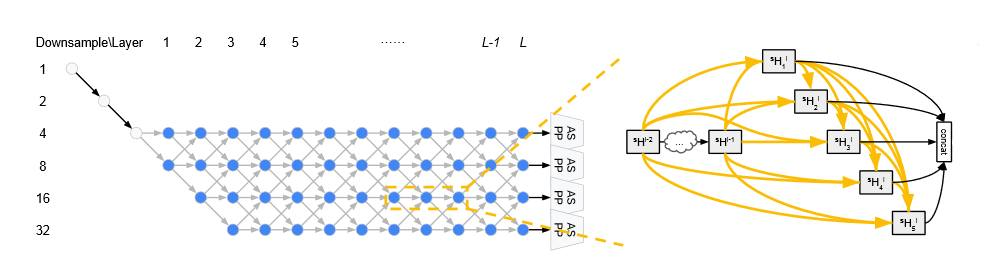
\includegraphics[width=1\textwidth]{Pictures/AutoDeepLab/Autodeeplab1.jpg}
	\caption{Auto-DeepLab Architektur. \cite{autodeeplabPaper}}
	\label{pic:autodeeplab_Architektur}
\end{figure}

Die drei Schritte (schräg nach oben, waagerecht, schräg nach unten), die durch die hellgrauen Pfeile dargestellt sind, können als Übergangswahrscheinlichkeiten von einem Zustand (einer Zelle) in den nächsten (nächste Zelle) interpretiert werden. Die drei Skalare sind somit alle nicht-negativ und bilden in der Summe einen Wert von 1. Als beste Architektur wird der Pfad bestimmt, der die Übergangswahrscheinlichkeiten maximiert.\\[0.3cm]
Rechts in Abbildung \ref{pic:autodeeplab_Architektur} sind insgesamt drei (blaue) Zellen dargestellt: Zelle $l-2$ ($\prescript{s}{}{H}^{l-2}$), Zelle $l-1$ ($\prescript{s}{}{H}^{l-1}$) und Zelle $l$ ($\prescript{s}{}{H}^{l}$). Zelle $l$ ist anders dargestellt als $l-1$ und $l-2$: Hier wird das Innere der Zelle, also die Blöcke, dargestellt. Bei Auto-DeepLab besteht jede Zelle aus genau 5 Blöcken. Wie bereits oben beschrieben, bestehen die möglichen Inputs eines Blocks aus den Outputs der zwei Vorgängerzellen und den Outputs der Vorgängerblöcke in der Zelle $l$. Das hochgestellte $s$ steht für die Stufe an Downsamplings, also $s \in \{4,8,16,32\}$ (es wird bei 4 angefangen, da initial bereits zwei Downsamplings durchgeführt werden).\\[0.3cm]
Zwei beispielhafte, gefundene Architekturen sind in Abbildung 3.2 dargestellt.\\

\begin{figure}[H]
	\centering
	\begin{subfigure}[b]{0.47\textwidth}
		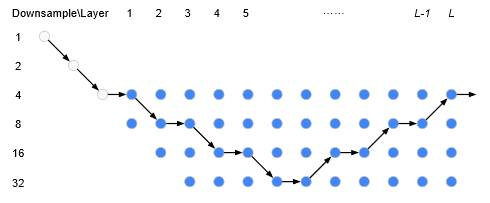
\includegraphics[width=\textwidth]{Pictures/AutoDeepLab/Autodeeplab2.jpg}
		\caption{Netz Architektur verwendet für Conv-Deconv \cite{conv_deconv} }
		\label{pic:autodeeplabBsp1}
	\end{subfigure} \hfill
	\begin{subfigure}[b]{0.47\textwidth}
		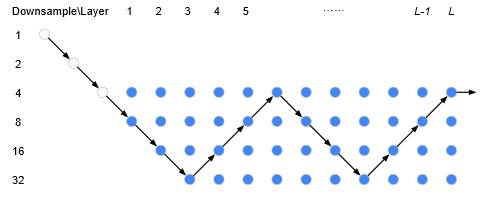
\includegraphics[width=\textwidth]{Pictures/AutoDeepLab/Autodeeplab3.jpg}
		\caption{Netz Architektur verwendet für Stacked Hourglass \cite{stacked_hourglass}}
		\label{pic:autodeeplabBsp2}
	\end{subfigure}
	\caption{Architekturen ermittelt durch Auto-DeepLab für zwei verschiedene Bilddatensätze. \cite{autodeeplabPaper} }
\end{figure}

In Abbildung \ref{pic:autodeeplabBsp1} sieht man eine fast U-förmige Architektur. Diese Form werden wir spezifischer und - anders als hier - bewusst forciert bzw. angewandt in Kapitel \ref{ch:nnunet} zum nnU-Net genauer betrachten. Beide hier dargestellten Architekturen enden auf Stufe 4 der Downsamplings (was allerdings keineswegs immer der Fall ist). Damit die Auflösung des Eingabebildes zurückgewonnen werden kann, folgen auf jeder Downsampling Stufe nach der L-ten Schicht die sogenannten Atrous Spatial Pyramid Pooling Module (in Abbildung \ref{pic:autodeeplab_Architektur} als ASPP abgekürzt). Mit Hilfe dieser Module wird durch Upsampling die ursprüngliche Auflösung wieder gewonnen.\\[0.3cm]
Für die Suche nach der perfekten Architektur nutzt Auto-DeepLab 40 Epochen. Die Batch-Größe beträgt 2. Wie bereits erwähnt, wird mit Gradient Descent gearbeitet. Genauer wird Stochastic Gradient Descent angewandt, um schneller Ergebnisse erzielen zu können. Gestartet wird mit einer Lernrate von 0.025, diese reduziert sich allerdings im Verlauf der Suche immer weiter bis schließlich auf einen Wert von 0.001.\\
Auffällig ist, dass in den ersten $75\%$ der Layer (also in den ersten 9 Layer) eher Downsampling dominiert und in den letzten $25\%$ (also letzten 3 Layer) eher Upsampling stattfindet.\\
Zudem ist zu bemerken, dass atrous und depthwise convolution häufig gewählt werden als Operatoren aus $\mathcal{O}$.

\section{Unsere Arbeit / Praxis}

Nachdem wir uns mit der Theorie von Auto-DeepLab auseinander gesetzt hatten, haben wir versucht, das Programm zum Laufen zu bringen. Der Datensatz, den wir zur Verfügung hatten und mit Hilfe von Auto-DeepLab segmentieren wollten, ist ein Datensatz \cite{larven}, welcher Larven \todo{Was für Larven, welche Quelle, wie Larven sichtbar gemacht?} darstellt: Er beinhaltet Graustufen-Bilder von Larven auf einer Glasscheibe, die mittels Frustrated Total Internal Reflection abgelichtet wurden. Ziel war es, die Larven zu segmentieren und die Verschmutzungen um die Larven herum dabei zu ignorieren. Die Larven im Bild sind hell zu sehen. Der Hintergrund ist schwarz und nimmt einen sehr großen Teil der Bilder ein (über $90\%$). Somit ist der Anteil der zu segmentierenden Objekte, also hier die Larven, sehr klein. Um das Programm auszuführen, haben wir den Link in dem Paper \cite{autodeeplabPaper} auf Seite 1 unten genutzt, der zu einem GitHub Repository führt. Allerdings ist uns aufgefallen, dass der Link zu dem Repository zu $\textit{DeepLab}$ führt \cite{deeplabGithub}, und somit nicht zu einer Veröffentlichung von $\textit{Auto-DeepLab}$, was uns sehr verwundert hat \todo{mit der Verwunderung rausnehmen?} , nachdem uns das aufgefallen ist. So haben wir also mit DeepLab und nicht, mit Auto-DeepLab gearbeitet. Nach anfänglichen Schwierigkeiten haben wir es letztlich geschafft, das Programm auf dem Larven-Datensatz zum Laufen zu bringen mit Hilfe des Checkpoints, der auf der GitHub Seite zu finden ist. Allerdings wurde jedes Bild ausschließlich als schwarz segmentiert. Da der Hintergrund der Bilder einen sehr großen Teil der Bilder einnimmt, waren die Ergebnisse was den Score angeht nicht gänzlich schlecht. Aber das wirklich brauchbare Ergebnis war natürlich sehr schlecht: Wenn jedes Bild als schwarzes Bild segmentiert wird, existiert kein Mehrwert.\\
Da aber die Objekte nur einen sehr kleinen Anteil der Bilder einnehmen, haben wir den Ansatz verfolgt, die Bilder in viele kleine Bilder zu zerschneiden (siehe Abbildung \ref{pic:zerschnitteneLarven}), sodass sich der Anteil der zu segmentierenden Objekte vergrößert. Wir hatten die Hoffnung, dass das Programm die Larven dann erkennt und so in der Lage ist, die Larven zu segmentieren. So haben wir die Bilder zerschnitten zu vielen kleinen Bildern.\\
Leider hat das aber keine Wirkung gezeigt: Noch immer wurden ausschließlich schwarze Bilder ausgegeben. Die Larven konnten also nicht segmentiert werden.\\
In den GitHub Issues konnten wir leider keine Lösung unseres Problems finden. Im Gegenteil haben wir dort mehrere Beiträge gefunden, die zeigen, dass scheinbar viele andere Nutzer ebenfalls (ähnliche) Probleme wie wir hatten.\\

\begin{figure}[H]
	\centering
	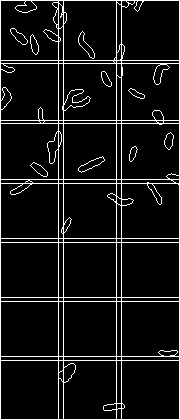
\includegraphics[width=0.15\textwidth]{Pictures/AutoDeepLab/ZerschnittBoxen-Beispiel.png}
	\caption{Zerschnittene Larvenbilder in der Übersicht.}
	\label{pic:zerschnitteneLarven}
\end{figure}

Als weiteren Versuch, mit Hilfe von Auto-DeepLab, die Larven zu segmentieren, sind wir auf die GitHub Seite von Noam Rosenberg \cite{deeplabRosenberg} gestoßen. Hier scheint die vielleicht sogar einzige Implementierung von Auto-DeepLab zu existieren. So haben wir uns mit dieser Umsetzung beschäftigt. Da es uns aber viel zu aufwendig erschien, sich dort weiter hineinzuarbeiten, haben wir den Versuch, mit Hilfe von Auto-DeepLab Bilder zu segmentieren, an dieser Stelle beendet.

\section{Ergebnisse}

Wie bereits in dem vorherigen Unterabschnitt zu dem Praxisteil zu Auto-DeepLab beschrieben, waren unsere Ergebnisse nicht zu gebrauchen. Da jedes Bild ausschließlich als schwarz ausgegeben wurde, sind die Ergebnisse als sehr schlecht zu bewerten, bzw. der Versuch, Ergebnisse zu erzielen, ist gescheitert. Auch der Ansatz, den Anteil der zu segmentierenden Objekte im Bild zu vergrößern durch das Zerschneiden der Bilder, hat nichts gebracht.\\
Wir vermuten, dass der in GitHub angegebene Checkpoint nicht geeignet ist.

\section{Fazit}

Auto-DeepLab verfolgt einen interessanten Ansatz, Bilder zu segmentieren. In der Theorie wird Auto-DeepLab für die sehr geringe Trainings- / Suchzeit gelobt. Auffällig ist jedoch, dass der Link in dem Paper zu Auto-DeepLab \cite{autodeeplabPaper} zu einer Umsetzung von DeepLab \cite{deeplabGithub} führt.  So haben wir damit gearbeitet, konnten allerdings keine Ergebnisse erzielen und haben bei der Suche nach Lösungen festgestellt, dass viele Andere ebenfalls Probleme hatten, mit dem Framework zu arbeiten.

